\chapter{Sequenzdiagramm}

Im Folgenden wird der Vorgang eines vollständigen Buchungsdurchgangs betrachtet, um final mittels Sequenzdiagrammen das Vorgehen visuell darzustellen.

Bei der Erarbeitung wird aufgrund des Umfangs ein Teil der Detailtiefe entfernt. Die exakte Kommunikation mit der Datenbasis (in Realität mit einer Datenbank und im Projekt mit den CSV-Dateien) wird nicht betrachtet. Bei der Interaktion mit der Anwendung wird die Unterteilung in verschiedene GUIs unter dem Begriff 'Benutzeroberfläche' zusammengefasst. Es wird ebenfalls davon ausgegangen, dass für den Sequenzablauf benötigte Datensätze wie Fahrzeuge, Standorte, Kunden und Mitarbeiter bereits vorhanden sind und nicht erst angelegt werden müssen. Davon auszugehen, dass mit einer vollständig leeren Datenbasis begonnen wird ist für die Abbildung des Buchungsablaufs nicht zielführend. Aus diesem Grund wird angenommen, dass ausschließlich die Datenbasis der Buchungen, Rechnungen und Mahnungen leer ist. Weiterhin wird in den Sequenzdiagrammen auf die Verwendung von Funktionen verzichtet und Vorgänge werden umschrieben oder umgangssprachlich aufgeführt.

\section{Aktionsbetrachtung: Buchung eines Fahrzeugs}

Eine Buchung soll angelegt werden. Abgesehen vom eigentlichen Buchungsdurchgangs soll auch die Abrechnung des Buchungstermins einbezogen werden. Ausgehend davon lassen sich mehrere Teil-Abläufe identifizieren: Buchung eines Fahrzeugs, Stornierung einer Buchung, Antreten des gebuchten Termins, Beendigung der Fahrt mit Erstellung einer Rechnung und notfalls Mahnungen. Die Buchung und die Stornierung lassen sich zusammenfassen, gleiches gilt für die Beendigung und die Rechnungsausstellung. Da die Buchung über die Desktopanwendung ausschließlich in der Filiale stattfinden kann, ist ein Akteur der Organisator, der zweite Aktuer ist der Kunde.


Der gesamte Buchungsvorgang beginnt damit, dass ein Kunde die Filiale betritt und einen Termin buchen möchte. Sobald der Kunde einen Terminwunsch und die damit verbundenen Bedinungen (Fahrzeug, Zeitraum, Standort) formuliert, kann der Organisator diese Daten in die Benutzeroberfläche eingeben und die Eingabe validieren lassen. Das System meldet anschließend zurück, ob die Eingabekombination buchbar ist oder nicht.


Die Stornierung eines gebuchten Termins ist bis zu 10 Stunden vor Antritt möglich. Um einen Termin stornieren zu können, muss der Kunde telefonisch oder in Person die Stornierung beim Organisator anfragen. Dieser filtert nach dem Kunden und wählt die betroffene Buchung aus. Sobald die richtige Buchung gefunden wurde, kann sie gelöscht werden.


Beim Terminantritt muss der Kunde seine Kundekarte dem Kartenlesegerät präsentieren, welches zum gebuchten Fahrzeug gehört. Der darin enthaltene Mini-Controller vergleicht die in der Karte enthaltenen Kundendaten mit den Daten in der Datenbasis. Sofern für den Kunden eine Buchung hinterlegt ist, bei der das Fahrzeug und die Zeit übereinstimmen, wird das Fahrzeug vom Controller entsperrt.


Nach der finalen Abgabe überprüft der Controller den Kilometerstand und verriegelt anschließend das Fahrzeug. Serverseitig wird nun der neue Kilometerstand mit dem alten Stand verglichen und daraus wird die gefahrene Kilometeranzahl berechnet. Auf Basis der Buchung (enthält gebuchtes Fahrzeug, welches wieder auf die Preiskalssen verweist) und den Kilometern wird ein Rechnungsobjekt erstellt. Letztendlich erhält der Kunde per E-Mail einen visuellen Export des Rechnungsobjekts.


Der Kunde hat nun standardmäßig 30 Tage Zeit, um die Rechnung zu zahlen. Sollte die Frist versäumt werden, wird die erste Mahnung erstellt und dem Kunden zugesandt. Nach 45 Tagen erfolgt die zweite Mahnung. Sollte nach zwei Monaten die Rechnung immer noch ausstehend sein, wird das betroffene Kundenkonto gesperrt und rechtliche Schritte werden eingeleitet.

\section{Pseudo-Code}

-to be continued-

\section{Diagramme}

\subsection{Buchung anlegen}


Das Anlegen einer Buchung wird in Abbildung \ref{img:buchung01} auf Seite \pageref{img:buchung01} dargestellt. Die Sequenz beginnt damit, dass der Kunde einen Terminwunsch gegenüber einem Mitarbeiter äußert. Der Organisator öffnet daraufhin das Formular für das Anlegen einer Buchung und teilt dem Kunden mit, dass die Buchung nun entgegengenommen werden kann.

Für die eigentliche Buchung nennt der Kunde dem Organisator zuerst den Zeitraum, den Standort und das Fahrzeug. Der Organisator trägt diese Daten in das Formular ein und klickt anschließend auf 'Buchung überprüfen'. Daraufhin lädt die Anwendung die Fahrzeug-, Standort- sowie Buchungsdaten und gleicht diese mit der Eingabe des Organisators ab. Falls es eine Kollision mit einer anderen Buchung gibt, wird die Buchung abgebrochen. In diesem Fall nennt der Kunde andere Buchungsdaten, bis es keine Kollision mehr gibt. Sollte es keine Kollision geben, wird die Buchung in der Datenbasis hinterlegt und das System bestätigt die Buchung. Daraufhin teilt der Organisator dem Kunden mit, dass die Buchung erfolgreich war.

Optional kann der Kunde die Buchung nun stornieren. Dazu muss der Kunde gegenüber dem Organisator den Wunsch äußern, die Buchung zu stornieren. Der Organisator erfagt daraufhin den Namen des Kunden und gibt diesen in der entsprechenden Suchleiste ein. Die Anwendung lädt daraufhin die Kundendaten aus der Datenbasis und zeigt sie dem Organisator an. Im Anschluss erfagt der Organisator, welche Buchung der Kunde gern stornieren möchte. Nachdem der Kunde die Buchung spezifiziert hat, wählt der Organisator die entsprechende Buchung aus. Daraufhin lädt die Anwendung die Buchungsdaten für die spezifizierte Buchung aus der Datenbasis und zeigt diese Daten an. Der Organisator klickt anschließend auf 'Buchung stornieren', wodurch die Buchung aus der Datenbasis gelöscht wird. Der Organisator erhält darufhin eine Bestätigung für das Löschen der Buchung und teilt dem Kunden mit, dass die Buchung erfolgreich storniert wurde. 

\newpage

\begin{figure}[!ht]
    \centering
    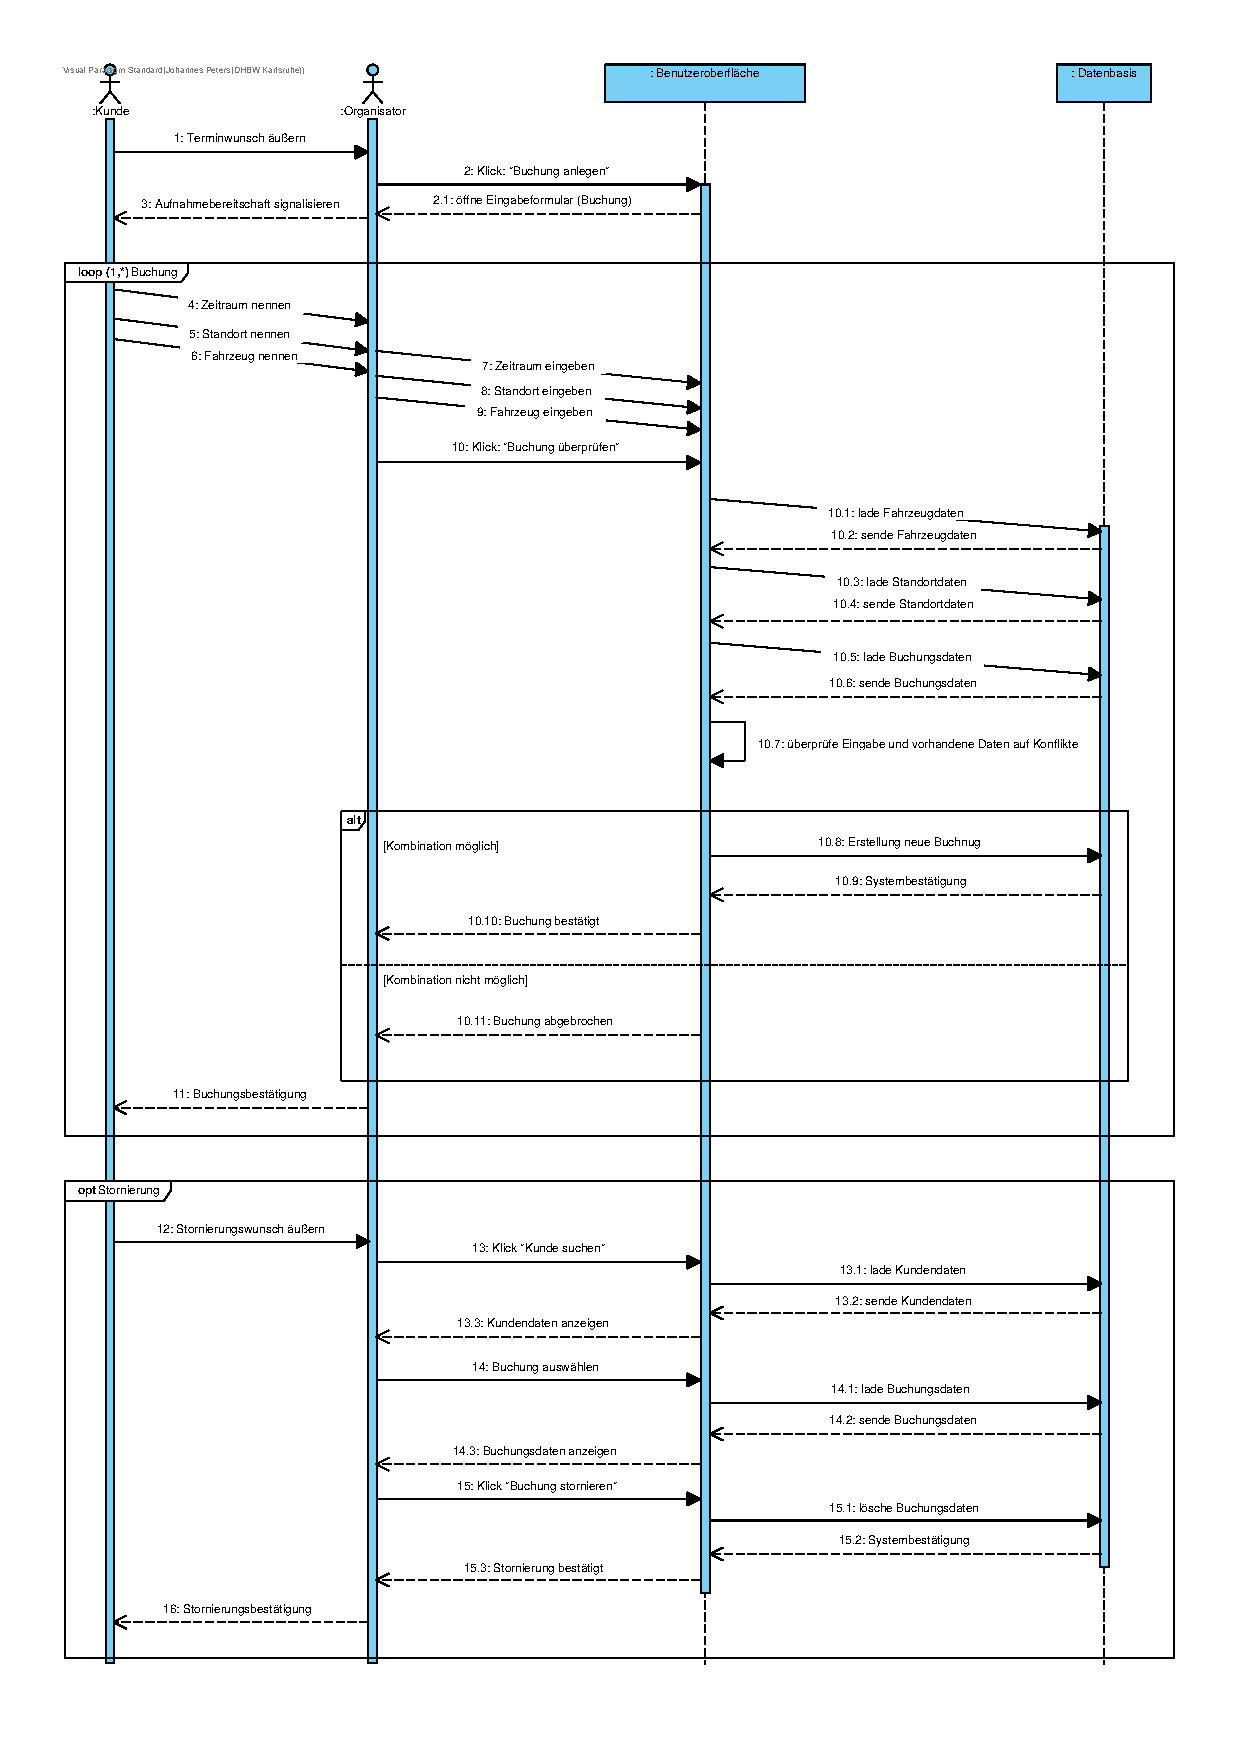
\includegraphics[width=\textwidth, height=\textheight-4cm]{Bilder/Diagramme/SD_Buchungsvorgang_01.pdf}
    \caption{Buchung eines Termins}
    \label{img:buchung01}
\end{figure}


\clearpage

\subsection{Fahrt antreten}

Das Antreten einer Fahrt wird in Abbildung \ref{img:buchung02} auf Seite \pageref{img:buchung02} dargestellt. Hierbei lässt der Kunde zuerst seine Kundenkarte vom Lesegerät einscannen, welches die Kundendaten ausliest und im Anschluss die Buchungsdaten aus der Datenbasis lädt. Nachdem die Buchungsdaten geladen wurden wird zunächst der Standort überprüft, bevor die Kundendaten mit den Buchungsdaten abgeglichen werden. Bei einer übereinstimmung wird zuerst der Kilometerstand für die Abrechnung gespeichert und danach wird das Fahrzeug entriegelt. Nun kann der Kunde seine Fahrt beginnen. 


\begin{figure}[!ht]
    \centering
    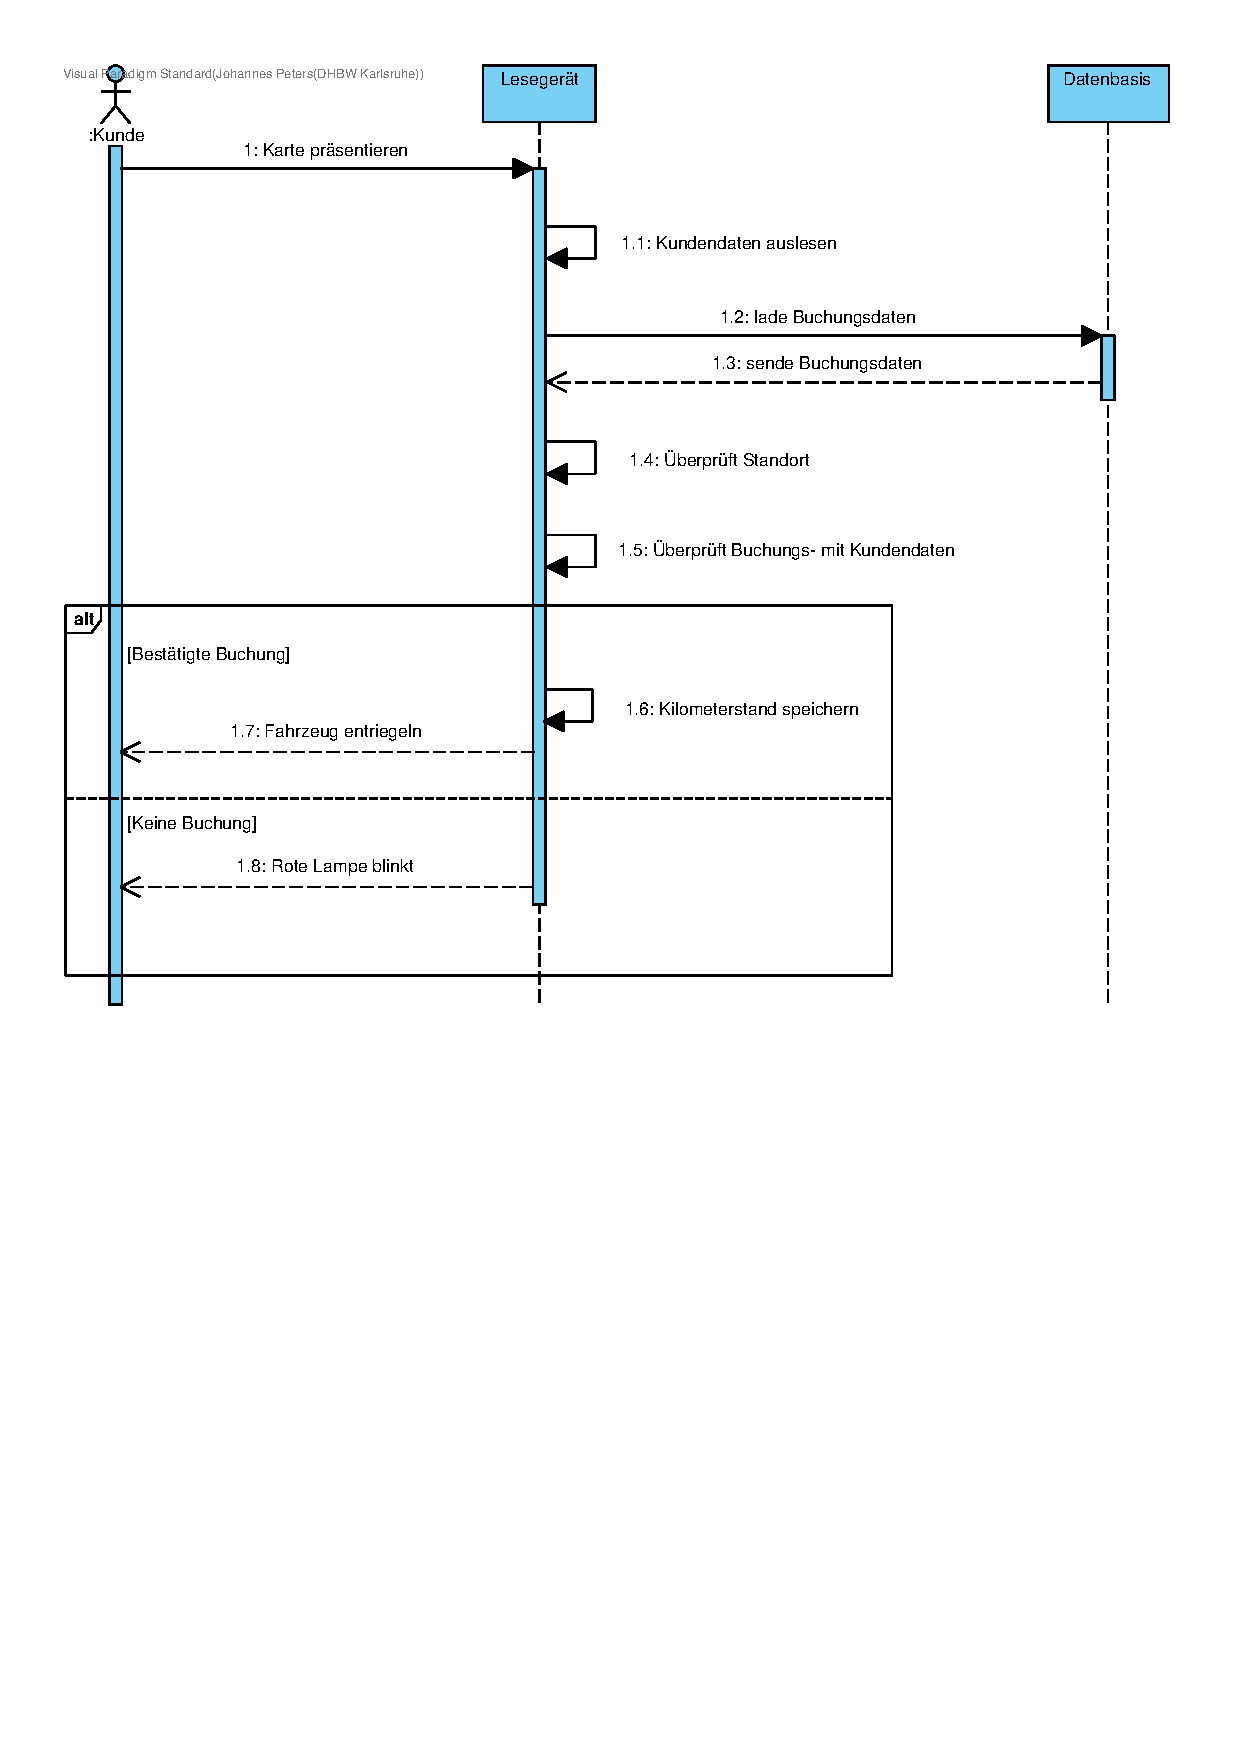
\includegraphics[width=\textwidth, trim = 0cm 13cm 0cm 0cm]{Bilder/Diagramme/SD_Buchungsvorgang_02.pdf}
    \caption{Antritt eines gebuchten Termins}
    \label{img:buchung02}
\end{figure}

\newpage

\subsection{Fahrt beenden}

Das Beenden einer Fahrt wird in Abbildung \ref{img:buchung03} auf Seite \pageref{img:buchung03} dargestellt. Sobald der Kunde das Fahrzeug abstellt wird der Kilometerstand vom Lesegerät abgefragt und das Fahrzeug wird verriegelt. Während der Kunde auf seine Rechnung wartet wird der neue Kilometerstand an den Server gesendet, welcher nach Abfrage des alten Kilometerstands und den Buchungsdaten die gefahrenen Kilometer berechnet. Basierend auf den Buchungsdaten und den gefahrenen Kilometern wird eine Rechnung erstellt, welche vom Server per Mail an den Kunden geschickt wird.


\begin{figure}[!ht]
    \centering
    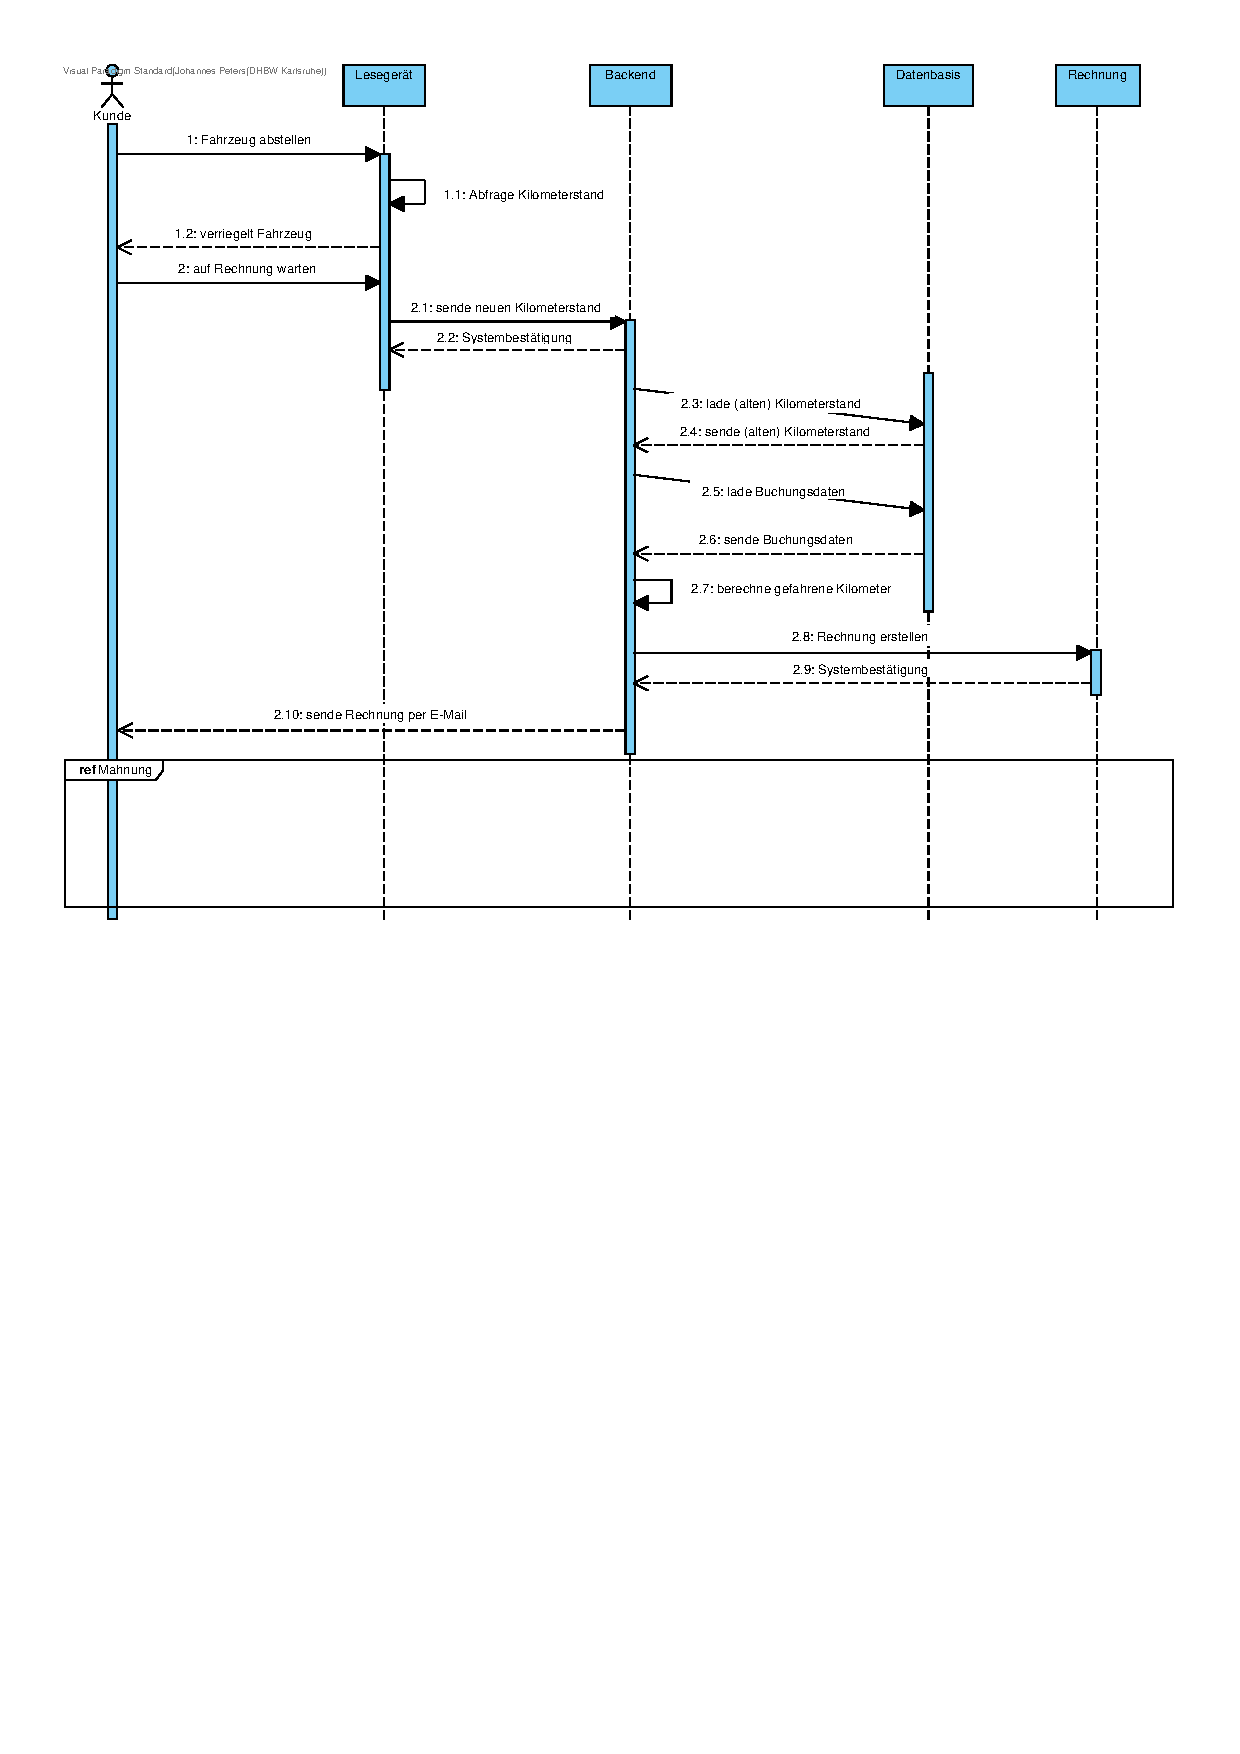
\includegraphics[width=\textwidth, trim = 0cm 14cm 0cm 0cm]{Bilder/Diagramme/SD_Buchungsvorgang_03.pdf}
    \caption{Abschluss eines gebuchten Termins}
    \label{img:buchung03}
\end{figure}

Falls die Rechnung vom Kunden ignoriert wird, erhält der Kunde nach 30 und nach 45 Tagen eine Mahnung. Dies wird in Abbildung \ref{img:buchung03} auf Seite \pageref{img:buchung03} dargestellt. Um eine Mahnung zu versenden lädt der Server zuerst die Rechnungsdaten der überfälligen Rechnung von der Datenbasis.
Im Anschluss erstellt der Server basierend auf der Rechnung eine Mahnung und sendet diese per Mail an den Kunden. Sollte der Kunde nach 60 Tagen nicht gezahlt haben, so wird er für vom Carsharing-Angebot ausgeschlossen. Dazu lädt der Server zuerst die Mahnungsdaten aus der Datenbasis, um den Status der Mahnung zu überprüfen. Wenn die Rechnung zu diesem Zeitpunkt nicht beglichen wurde, werden die Kundendaten aus der Datenbasis geladen und aktualisiert, sodass der Kunde für zukünftige Buchungen gesperrt ist. Sobald der Kunde blockiert ist sendet der Server eine Mail an den Kunden mit der Information, dass der Kunde in Zukunft vom Carsharing-Angebot ausgeschlossen ist und sein Schweizer Bankkonto eingefroren wurde.

\begin{figure}[!ht]
    \centering
    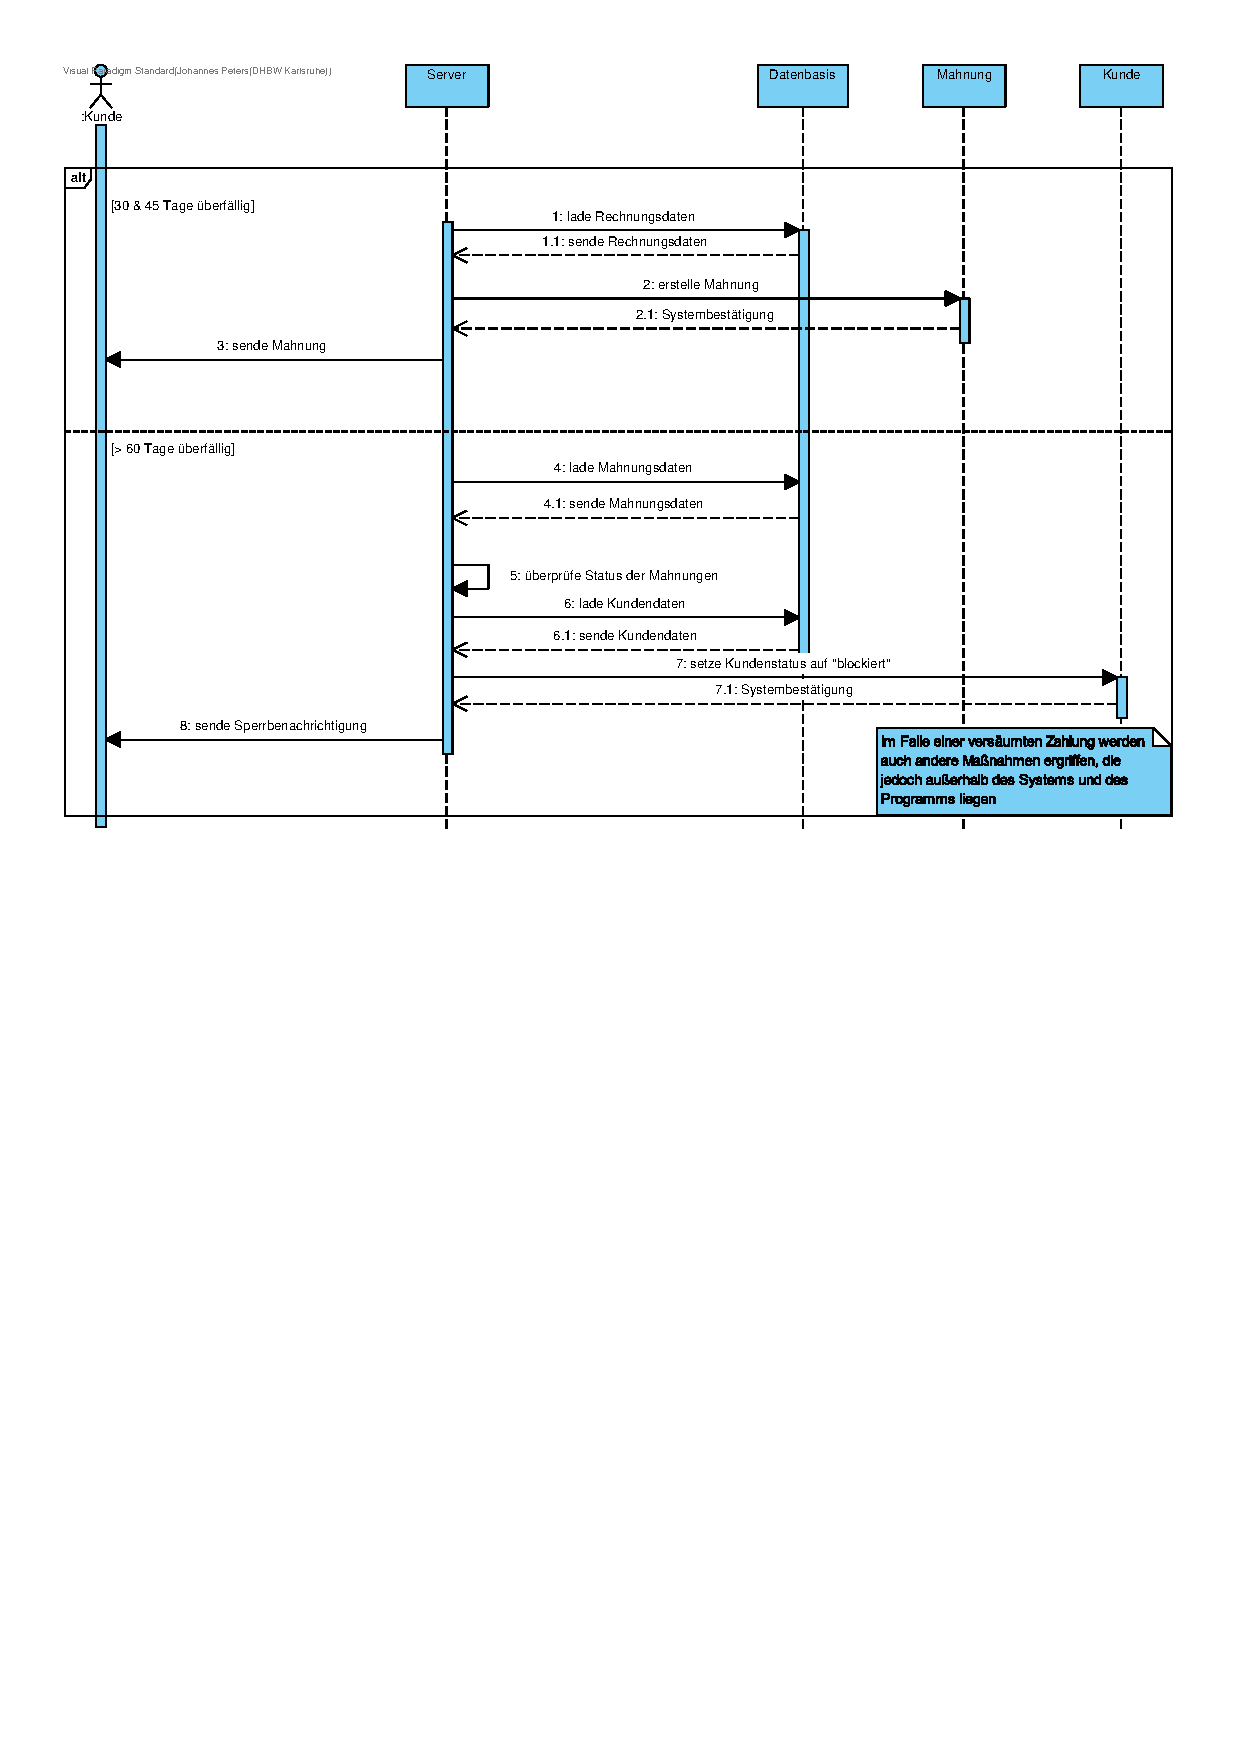
\includegraphics[width=\textwidth, trim = 0cm 16cm 0cm 0cm]{Bilder/Diagramme/SD_Buchungsvorgang_04.pdf}
    \caption{Erstellung der Mahnungen}
    \label{img:buchung04}
\end{figure}
